\section{Applications}

\subsection{Denoising}

\begin{description}
 \item[btkNLMDenoising] This program applies a non-local mean filter to a 3D image for denoising purpose. Usage: \texttt{-i input\_image\_filename -o output\_image\_filename}. The best results are usually obtained by using a mask (or a padding value).
\end{description}

\begin{description}
 \item[btkNLMDenoising4DImage] This program applies a non-local mean filter to each 3D image of a 4D image, for denoising purpose. Usage: \texttt{-i input\_image\_filename -o output\_image\_filename}. The best results are usually obtained by using a mask (or a padding value).
\end{description}


\subsection{Tractography}

    \subsubsection*{Executable presentation}
        \begin{description}
        \item[btkTractography] This program performs a probabilistic tractography using a particle filtering. Usage: \texttt{-d dwi\_image\_filename -v dwi\_gradient\_vectors -m white\_matter\_mask -l seeds\_la\-bel\_image}.
        \end{description}

    \subsubsection*{Standard usage}
        Suppose you want to perform a tractography on a diffusion weighted MRI dataset. You should have a dwi image, the corresponding gradient vectors' coordinates, a mask of the brain white matter and a label image of the seeds. Assume this data is stored in files named repsectively for instance \texttt{data.nii.gz}, \texttt{data.bvec}, \texttt{mask.nii.gz} and \texttt{seeds.nii.gz}. The tractography is accomplished by the command below.
            \begin{quote}
                \texttt{btkTractography -d data.nii.gz -v data.bvec -m mask.nii.gz -l seeds.nii.gz}
            \end{quote}
        When the program terminates its task, the probability connection map and the fibers estimation are saved in files respectively named \texttt{map.nii.gz} and \texttt{fibers.vtk}. The connection map is a volume image of probability intensities (\texttt{i.e.} intensities between 0 and 1) with the same origin, orientation and spacing as the diffusion weighted image. The fibers are polygonal data of VTK library in world coordinates. The standard pipeline of the program is shown in Fig.~\ref{btkTractography-fig:standard-pipeline}.
            \begin{figure}
                \centering
                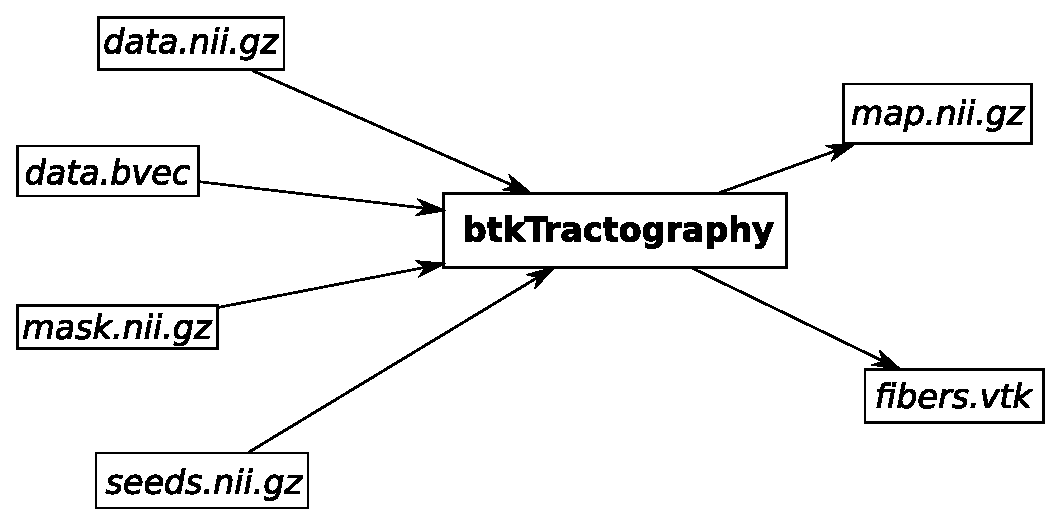
\includegraphics[width=0.6\textwidth]{btkTractographyPipeline}
                \caption{Standard pipeline of the btkTractography program.}
                \label{btkTractography-fig:standard-pipeline}
            \end{figure}

    \subsubsection*{Advanced usage}
        In addition to standard arguments of \texttt{btkTractography} program, there are some other parameters that let you to alter algorithm's behaviour. Since the default parameters values may work in the most of cases, they are optional. The program arguments are described below.
            \begin{description}
                \item[\texttt{-d --dwi}] Diffusion weighted sequence
                \item[\texttt{-v --vectors}] Gradient vectors' coordinates
                \item[\texttt{-m --mask}] White matter mask
                \item[\texttt{-l --label}] Seeds' label volume
                \item[\texttt{--angular-threshold}] Angular threshold between successive displacement vectors of a particle's trajectory
                \item[\texttt{--curve-constraint}] Curve constraint of particle's trajectory
                \item[\texttt{--step-length}] Step displacement's length of a particle
                \item[\texttt{--model-regularization}] Regularization coefficient of the model (\texttt{i.e.} regularization term of the model regression estimation)
                \item[\texttt{--model-order}] Order of the model (\texttt{i.e.} of spherical harmonics)
                \item[\texttt{-- --ignore\_rest}] Ignores the rest of the labeled arguments following this flag.
                \item[\texttt{--version}] Displays version information and exits.
                \item[\texttt{-h --help}] Displays usage information and exits.
            \end{description}

